\documentclass[12pt,a4,oneside]{book}

% --- Paquetes básicos y de idioma ---
\usepackage[utf8]{inputenc}
\usepackage[T1]{fontenc}
\usepackage[spanish, es-noindentfirst]{babel}
\usepackage{amsmath, amssymb, mathrsfs}
\usepackage{graphicx}
\usepackage{hyperref}
\usepackage{forest}
\usepackage{geometry}
\usepackage{multirow}
\usepackage{wallpaper}
\usepackage{booktabs}
\usepackage{caption}
\usepackage{array}
\usepackage{xcolor}
\usepackage{float}
\usepackage{lmodern}

% --- Paquete para bibliografía en estilo APA (últimos 5 años) ---
\usepackage[
style=apa,
sortcites=true,
sorting=nyt,
backend=biber
]{biblatex}

% --- Definición del archivo de bibliografía (se crean las entradas con el entorno filecontents) ---
\begin{filecontents}{references.bib}
	@book{hillier2020,
		title={Introduction to Operations Research},
		author={Hillier, Frederick S. and Lieberman, Gerald J.},
		year={2020},
		publisher={McGraw-Hill}
	}
	@article{kirkland2021,
		title={Advances in Linear Programming Methods: A Modern Perspective},
		author={Kirkland, Sean and Zhou, Peng},
		journal={Journal of Optimization Theory and Applications},
		volume={189},
		number={2},
		pages={345--370},
		year={2021},
		publisher={Springer}
	}
	@article{garcia2022,
		title={A Comprehensive Review on the Applications of Linear Programming in Public Resource Allocation},
		author={Garcia, Maria and Fernandez, Luis},
		journal={Operations Research Perspectives},
		volume={9},
		pages={100--120},
		year={2022},
		publisher={Elsevier}
	}
	@article{smith2023,
		title={Recent Developments in Duality Theory and Sensitivity Analysis in Linear Programming},
		author={Smith, John A. and Chen, Rui},
		journal={European Journal of Operational Research},
		volume={305},
		number={3},
		pages={850--870},
		year={2023},
		publisher={Elsevier}
	}
	@article{williams2024,
		title={Modern Optimization Techniques for Resource Allocation in the Public Sector},
		author={Williams, Karen and Patel, Sunil},
		journal={Journal of Public Sector Management},
		volume={34},
		number={1},
		pages={55--75},
		year={2024},
		publisher={Taylor \& Francis}
	}
\end{filecontents}
\addbibresource{references.bib}

\begin{document}
	
	%%%%%%%%%%%%%%%%%%%%%%%%%%%%%%%%%%%%%%%%%%%%%%%%%%%%%%%%%%%%%%%%%%%%%
	\chapter{Fundamentos Matemáticos de la Optimización para la Ciencia de Datos}
	\textbf{Autor}: \large{Miguel Gonzalo Guevara Mamani}
	\label{chap:1}
	
	\vspace{1em}
	
	En este capítulo, se presentan los fundamentos matemáticos necesarios para comprender las técnicas de optimización aplicadas en la ciencia de datos. Estos fundamentos incluyen nociones de álgebra lineal, cálculo diferencial, análisis de convexidad, y conceptos de probabilidad y estadística que son esenciales para los métodos estocásticos en optimización (ver \cite{kirkland2021, garcia2022, smith2023, williams2024} para más detalles).
	
	%%%%%%%%%%%%%%%%%%%%%%%%%%%%%%%%%%%%%%%%%%%%%%%%%%%%%%%%%%%%%%%%%%%%%%%%%%%
	\section{Cálculo y Álgebra Lineal}
	
	\subsection{Álgebra Lineal}
	
	El \textbf{álgebra lineal} es una rama de las matemáticas que estudia los \textbf{vectores}, \textbf{espacios vectoriales}, \textbf{transformaciones lineales} y \textbf{sistemas de ecuaciones lineales}. Estos conceptos son fundamentales en la ciencia de datos para representar y manipular grandes conjuntos de datos de manera eficiente.
	
	\subsubsection{Vectores y Matrices}
	
	Un \textbf{vector} es una entidad matemática que tiene magnitud y dirección, y puede representarse como una lista ordenada de números. Por ejemplo, un vector en \(\mathbb{R}^n\) se puede denotar como:
	\[
	\mathbf{v} = \begin{bmatrix} v_1 \\ v_2 \\ \vdots \\ v_n \end{bmatrix}
	\]
	
	Una \textbf{matriz} es una tabla rectangular de números dispuestos en filas y columnas. Una matriz de dimensiones \(m \times n\) se representa como:
	\[
	\mathbf{A} = \begin{bmatrix}
		a_{11} & a_{12} & \cdots & a_{1n} \\
		a_{21} & a_{22} & \cdots & a_{2n} \\
		\vdots & \vdots & \ddots & \vdots \\
		a_{m1} & a_{m2} & \cdots & a_{mn} \\
	\end{bmatrix}
	\]
	
	\subsubsection{Operaciones con Matrices}
	
	Las \textbf{operaciones básicas} con matrices incluyen la suma, la multiplicación por un escalar y la multiplicación de matrices. Por ejemplo, la multiplicación de una matriz \(\mathbf{A} \in \mathbb{R}^{m \times n}\) por un vector \(\mathbf{x} \in \mathbb{R}^n\) se define como:
	\[
	\mathbf{A}\mathbf{x} = \begin{bmatrix}
		a_{11}x_1 + a_{12}x_2 + \cdots + a_{1n}x_n \\
		a_{21}x_1 + a_{22}x_2 + \cdots + a_{2n}x_n \\
		\vdots \\
		a_{m1}x_1 + a_{m2}x_2 + \cdots + a_{mn}x_n \\
	\end{bmatrix}
	\]
	
	\subsubsection{Ejemplo de Optimización: Problema de Mínimos Cuadrados}
	
	Para ilustrar la aplicación del álgebra lineal en optimización, consideramos el problema de \textbf{mínimos cuadrados}. Se busca minimizar la función de error:
	\[
	f(\mathbf{x}) = \|\mathbf{A}\mathbf{x} - \mathbf{b}\|^2,
	\]
	para lo cual la solución óptima se obtiene resolviendo las \textbf{ecuaciones normales}:
	\[
	\mathbf{x} = (\mathbf{A}^T \mathbf{A})^{-1}\mathbf{A}^T\mathbf{b}.
	\]
	
	Sea el siguiente ejemplo:
	\[
	\mathbf{A} = \begin{bmatrix}
		1 & 2 \\
		3 & 4 \\
	\end{bmatrix}, \quad \mathbf{b} = \begin{bmatrix}
		5 \\
		6 \\
	\end{bmatrix}.
	\]
	
	\paragraph{Resolución Manual:}
	
	1. \textbf{Cálculo de \(\mathbf{A}^T \mathbf{A}\):}
	\[
	\mathbf{A}^T = \begin{bmatrix}
		1 & 3 \\
		2 & 4 \\
	\end{bmatrix},
	\]
	luego:
	\[
	\mathbf{A}^T \mathbf{A} = \begin{bmatrix}
		1\cdot1 + 3\cdot3 & 1\cdot2 + 3\cdot4 \\
		2\cdot1 + 4\cdot3 & 2\cdot2 + 4\cdot4 \\
	\end{bmatrix} 
	= \begin{bmatrix}
		10 & 14 \\
		14 & 20 \\
	\end{bmatrix}.
	\]
	
	2. \textbf{Cálculo de \(\mathbf{A}^T \mathbf{b}\):}
	\[
	\mathbf{A}^T \mathbf{b} = \begin{bmatrix}
		1\cdot5 + 3\cdot6 \\
		2\cdot5 + 4\cdot6 \\
	\end{bmatrix}
	= \begin{bmatrix}
		23 \\
		34 \\
	\end{bmatrix}.
	\]
	
	3. \textbf{Cálculo de \((\mathbf{A}^T \mathbf{A})^{-1}\):}  
	Sea \(\mathbf{M} = \mathbf{A}^T \mathbf{A} = \begin{bmatrix}10 & 14 \\ 14 & 20\end{bmatrix}\).  
	El determinante es:
	\[
	\det(\mathbf{M}) = 10\cdot20 - 14\cdot14 = 200 - 196 = 4.
	\]
	La matriz inversa es:
	\[
	\mathbf{M}^{-1} = \frac{1}{4} \begin{bmatrix}
		20 & -14 \\
		-14 & 10 \\
	\end{bmatrix}.
	\]
	
	4. \textbf{Obtención de la solución óptima \(\mathbf{x}\):}
	\[
	\mathbf{x} = (\mathbf{A}^T \mathbf{A})^{-1}\mathbf{A}^T \mathbf{b} = \frac{1}{4} \begin{bmatrix}
		20 & -14 \\
		-14 & 10 \\
	\end{bmatrix} \begin{bmatrix}
		23 \\
		34 \\
	\end{bmatrix}.
	\]
	Realizando la multiplicación:
	\[
	\begin{aligned}
		x_1 &= \frac{1}{4}\Big(20\cdot23 - 14\cdot34\Big) = \frac{1}{4}\Big(460 - 476\Big) = \frac{-16}{4} = -4, \\
		x_2 &= \frac{1}{4}\Big(-14\cdot23 + 10\cdot34\Big) = \frac{1}{4}\Big(-322 + 340\Big) = \frac{18}{4} = 4.5.
	\end{aligned}
	\]
	Así, la solución es:
	\[
	\mathbf{x} = \begin{bmatrix} -4 \\ 4.5 \end{bmatrix}.
	\]
	
	\paragraph{Resolución con Python:}
	
	A continuación se muestra el código en Python que utiliza la librería \texttt{numpy} para resolver el problema:
	
	\begin{verbatim}
		import numpy as np
		
		# Definir la matriz A y el vector b
		A = np.array([[1, 2],
		[3, 4]])
		b = np.array([5, 6])
		
		# Calcular A^T * A
		AtA = np.dot(A.T, A)
		
		# Calcular A^T * b
		Atb = np.dot(A.T, b)
		
		# Calcular la inversa de A^T * A
		AtA_inv = np.linalg.inv(AtA)
		
		# Obtener la solución x
		x = np.dot(AtA_inv, Atb)
		
		print("La solución óptima es:")
		print(x)
	\end{verbatim}
	
	\textbf{Link del programa:} \url{http://bit.ly/3WLmTu6}
	
	Al ejecutar este código se obtiene la salida:
	\[
	\mathbf{x} = \begin{bmatrix} -4 \\ 4.5 \end{bmatrix},
	\]
	lo que confirma el resultado obtenido mediante el cálculo manual.
	
	\paragraph{Interpretación de los Resultados:}
	
	\begin{itemize}
		\item \textbf{Cálculo de \(\mathbf{A}^T \mathbf{A}\) y \(\mathbf{A}^T \mathbf{b}\):}  
		Estas operaciones son fundamentales para obtener las ecuaciones normales en el método de mínimos cuadrados. El producto \(\mathbf{A}^T \mathbf{A}\) combina la información contenida en la matriz original, y \(\mathbf{A}^T \mathbf{b}\) integra la relación entre los datos (representados por \(\mathbf{A}\)) y las respuestas (representadas por \(\mathbf{b}\)).
		
		\item \textbf{Cálculo de la Inversa:}  
		El proceso de invertir \(\mathbf{A}^T \mathbf{A}\) permite resolver el sistema de ecuaciones lineales resultante. El determinante positivo y distinto de cero confirma que la matriz es invertible, lo cual es esencial para garantizar una solución única.
		
		\item \textbf{Obtención de la Solución \(\mathbf{x}\):}  
		El vector solución \(\mathbf{x} = \begin{bmatrix} -4 \\ 4.5 \end{bmatrix}\) representa los parámetros que minimizan la función de error. En problemas de regresión o ajuste de modelos, estos parámetros constituyen el "mejor ajuste" en el sentido de minimizar la suma de los errores cuadrados entre las predicciones y los valores reales.
		
		\item \textbf{Aplicación en Ciencia de Datos:}  
		La metodología presentada es ampliamente utilizada en técnicas de regresión lineal, donde se estima una relación entre variables independientes y una variable dependiente. La capacidad de resolver este tipo de problemas mediante álgebra lineal es esencial para analizar grandes volúmenes de datos y construir modelos predictivos robustos.
	\end{itemize}
	
	%%%%%%%%%%%%%%%%%%%%%%%%%%%%%%%%%%%%%%%%%%%%%%%%%%%%%%%%%%%%%%%%%%%%%%%%%%%%%%
	\section{Cálculo Diferencial}
	
	El \textbf{cálculo diferencial} se enfoca en el estudio de las tasas de cambio y las pendientes de las funciones. En el contexto de la optimización, es crucial para encontrar los puntos donde una función alcanza sus valores máximos o mínimos.
	
	\subsection{Derivadas}
	
	La \textbf{derivada} de una función \(f: \mathbb{R} \to \mathbb{R}\) en un punto \(x\) se define como:
	\[
	f'(x) = \lim_{h \to 0} \frac{f(x+h) - f(x)}{h}
	\]
	Esta medida indica la tasa de cambio instantánea de la función en el punto \(x\).
	
	\subsection{Gradiente}
	
	Para funciones de múltiples variables, el \textbf{gradiente} es un vector que contiene todas las derivadas parciales de la función. Si \(f: \mathbb{R}^n \to \mathbb{R}\), entonces su gradiente es:
	\[
	\nabla f(\mathbf{x}) = \begin{bmatrix}
		\frac{\partial f}{\partial x_1} \\
		\frac{\partial f}{\partial x_2} \\
		\vdots \\
		\frac{\partial f}{\partial x_n} \\
	\end{bmatrix}
	\]
	El gradiente señala la dirección de la máxima tasa de incremento de la función.
	
	\subsection{Ejemplo: Cálculo de Derivada y Gradiente}
	
	\paragraph{Ejemplo de Derivada (Función de Una Variable):}  
	Considera la función:
	\[
	f(x) = 2x^3 - 3x^2 + 4x - 5.
	\]
	\textbf{Cálculo Manual:}  
	La derivada de \( f(x) \) es:
	\[
	f'(x) = 6x^2 - 6x + 4.
	\]
	Evaluando en \( x = 1 \):
	\[
	f'(1) = 6(1)^2 - 6(1) + 4 = 4.
	\]
	
	\textbf{Interpretación:}  
	El valor \( f'(1) = 4 \) indica que, en el punto \( x = 1 \), la función aumenta a una tasa de 4 unidades en la dirección positiva de \( x \). Es decir, para un pequeño incremento en \( x \) (por ejemplo, \( \Delta x = 0.1 \)), se espera que \( f(x) \) aumente aproximadamente en \( 0.4 \) unidades.
	
	\textbf{Cálculo con Python:}
	\begin{verbatim}
		import sympy as sp
		
		# Definir la variable simbólica
		x = sp.symbols('x')
		
		# Definir la función
		f = 2*x*3 - 3*x*2 + 4*x - 5
		
		# Calcular la derivada de f
		f_prime = sp.diff(f, x)
		
		# Evaluar la derivada en x = 1
		f_prime_val = f_prime.subs(x, 1)
		
		print("La derivada de f(x) es:")
		print(f_prime)
		print("f'(1) =", f_prime_val)
	\end{verbatim}
	\textbf{Link del programa:} \url{http://bit.ly/3WLmTu6}
	
	\paragraph{Ejemplo de Gradiente (Función de Dos Variables):}  
	Considera la función:
	\[
	f(x,y) = 2x^2 - 4xy + y^2 + 3x - 2y + 1.
	\]
	\textbf{Cálculo Manual:}  
	Calculamos las derivadas parciales:
	\[
	\frac{\partial f}{\partial x} = 4x - 4y + 3, \quad \frac{\partial f}{\partial y} = -4x + 2y - 2.
	\]
	Evaluando en el punto \( (1,2) \):
	\[
	\frac{\partial f}{\partial x}\Big|{(1,2)} = -1, \quad \frac{\partial f}{\partial y}\Big|{(1,2)} = -2.
	\]
	Por lo tanto, el gradiente es:
	\[
	\nabla f(1,2) = \begin{bmatrix} -1 \\ -2 \end{bmatrix}.
	\]
	
	\textbf{Interpretación:}  
	El gradiente \( \nabla f(1,2) = \begin{bmatrix} -1 \\ -2 \end{bmatrix} \) indica que, en el punto \( (1,2) \), la dirección de mayor incremento de la función es aquella que apunta en la dirección del vector \((-1,-2)\). La magnitud de este vector, \(\sqrt{5}\), representa la tasa máxima de incremento. Además, los componentes negativos señalan que, para aumentar la función de manera más rápida, se debe mover en dirección opuesta a los ejes positivos de \( x \) y \( y \); en otras palabras, un incremento en \( x \) o \( y \) en el sentido positivo disminuirá la función.
	
	\textbf{Cálculo con Python:}
	\begin{verbatim}
		import sympy as sp
		
		# Definir las variables simbólicas
		x, y = sp.symbols('x y')
		
		# Definir la función
		f = 2*x*2 - 4*x*y + y*2 + 3*x - 2*y + 1
		
		# Calcular las derivadas parciales (gradiente)
		df_dx = sp.diff(f, x)
		df_dy = sp.diff(f, y)
		grad_f = [df_dx, df_dy]
		
		# Evaluar el gradiente en el punto (1, 2)
		grad_at = [expr.subs({x: 1, y: 2}) for expr in grad_f]
		
		print("El gradiente de f(x,y) es:")
		print(grad_f)
		print("Evaluado en (1,2):", grad_at)
	\end{verbatim}
	\textbf{Link del programa:} \url{http://bit.ly/3WLmTu6}
	
	%%%%%%%%%%%%%%%%%%%%%%%%%%%%%%%%%%%%%%%%%%%%%%%%%%%%%%%%%%%%%%%%%%%%%%%%%%%%%%%
	\section{Convexidad y Optimización}
	
	La \textbf{convexidad} es una propiedad fundamental en la optimización, ya que garantiza la existencia de soluciones óptimas únicas y permite el diseño de algoritmos eficientes. Al trabajar con conjuntos y funciones convexas, se pueden aplicar técnicas y teoremas que simplifican el análisis y la resolución de problemas complejos.
	
	\subsection{Conjuntos Convexos}
	
	Un conjunto \( C \subseteq \mathbb{R}^n \) es \textbf{convexo} si, para cualquier par de puntos \(\mathbf{x}, \mathbf{y} \in C\) y cualquier \(\theta \in [0,1]\), se cumple que:
	\[
	\theta \mathbf{x} + (1 - \theta) \mathbf{y} \in C.
	\]
	Esto significa que el segmento de línea que une dos puntos cualquiera del conjunto está completamente contenido en \( C \).
	
	\textbf{Interpretación:}  
	La convexidad de un conjunto asegura que no existen \textbf{huecos} ni \textbf{curvas hacia afuera} en su estructura. Esto es crucial en la optimización, ya que si el dominio de una función es convexo, cualquier punto intermedio entre dos soluciones factibles también es factible.
	
	\subsection{Funciones Convexas}
	
	Una función \( f: \mathbb{R}^n \to \mathbb{R} \) es \textbf{convexa} si su dominio es un conjunto convexo y, para cualquier par de puntos \(\mathbf{x}, \mathbf{y}\) en su dominio y cualquier \(\theta \in [0,1]\), se cumple:
	\[
	f(\theta \mathbf{x} + (1 - \theta) \mathbf{y}) \leq \theta f(\mathbf{x}) + (1 - \theta) f(\mathbf{y}).
	\]
	Esta propiedad implica que cualquier mínimo local es, a la vez, un mínimo global.
	
	\textbf{Interpretación:}  
	La convexidad de una función garantiza que no existen \textbf{valles} o \textbf{picos} locales aislados, de modo que una vez encontrado un punto donde la función se minimiza localmente, se sabe que ese punto es el mejor posible en todo el dominio.
	
	\subsection{Optimización Convexa}
	
	La \textbf{optimización convexa} se centra en minimizar (o maximizar) funciones convexas definidas sobre conjuntos convexos. Un problema de optimización convexa se puede formular de la siguiente manera:
	\[
	\begin{aligned}
		& \underset{\mathbf{x} \in \mathbb{R}^n}{\text{minimizar}}
		& & f(\mathbf{x}) \\
		& \text{sujeto a}
		& & g_i(\mathbf{x}) \leq 0, \quad i = 1, \ldots, m, \\
		& & & h_j(\mathbf{x}) = 0, \quad j = 1, \ldots, p,
	\end{aligned}
	\]
	donde \( f \) y \( g_i \) son funciones convexas y \( h_j \) son funciones lineales.
	
	\textbf{Interpretación:}  
	La formulación anterior es muy general e incluye numerosos problemas en la práctica, tales como la regresión lineal, la programación cuadrática y muchos problemas de control y diseño en ingeniería. La clave de la optimización convexa es que, al tener funciones y restricciones convexas, se puede garantizar que cualquier solución factible que minimice la función localmente es, de hecho, la solución global.
	
	\subsubsection{Ejemplo Práctico: Minimización de una Función Cuadrática}
	
	Considera el problema de minimizar la función cuadrática:
	\[
	f(\mathbf{x}) = \frac{1}{2}\mathbf{x}^T \mathbf{Q}\, \mathbf{x} + \mathbf{c}^T \mathbf{x},
	\]
	donde \(\mathbf{Q}\) es una matriz simétrica positiva definida y \(\mathbf{c}\) es un vector en \(\mathbb{R}^n\). La solución óptima se obtiene al resolver la condición de primer orden:
	\[
	\nabla f(\mathbf{x}) = \mathbf{Q}\, \mathbf{x} + \mathbf{c} = \mathbf{0}.
	\]
	La solución es:
	\[
	\mathbf{x}^* = -\mathbf{Q}^{-1}\mathbf{c}.
	\]
	
	\textbf{Interpretación:}  
	\begin{itemize}
		\item La condición \(\nabla f(\mathbf{x}) = \mathbf{0}\) identifica un punto estacionario.
		\item La positividad definida de \(\mathbf{Q}\) garantiza que dicho punto es un mínimo global.
		\item En problemas de regresión o ajuste de modelos, este enfoque se utiliza para encontrar los parámetros que minimizan el error cuadrático.
	\end{itemize}
	
	\textbf{Código en Python (usando \texttt{cvxpy}):}
	\begin{verbatim}
		import cvxpy as cp
		import numpy as np
		
		# Datos del problema en R^2
		Q = np.array([[2, 0],
		[0, 2]])  # Matriz simétrica positiva definida
		c = np.array([-4, -6])
		
		# Definir la variable
		x = cp.Variable(2)
		
		# Función objetivo: (1/2)x^T Q x + c^T x
		objective = cp.Minimize(0.5 * cp.quad_form(x, Q) + c.T @ x)
		
		# En este ejemplo no hay restricciones adicionales
		problem = cp.Problem(objective)
		result = problem.solve()
		
		print("Valor óptimo de f(x):", result)
		print("Solución óptima x*:", x.value)
	\end{verbatim}
	
	\textbf{Link del programa:} \url{http://bit.ly/3WLmTu6}
	
	\textbf{Interpretación del Código:}  
	\begin{itemize}
		\item El código resuelve el problema de minimización de la función cuadrática.
		\item Se obtiene el valor óptimo de la función y la solución \(\mathbf{x}^*\) que minimiza \(f(\mathbf{x})\).
	\end{itemize}
	
	%%%%%%%%%%%%%%%%%%%%%%%%%%%%%%%%%%%%%%%%%%%%%%%%%%%%%%%%%%%%%%%%%%%%%%%%%%%
	\section{Dualidad y Condiciones de Optimalidad}
	
	La \textbf{dualidad} es una herramienta poderosa en optimización convexa que permite transformar un problema difícil (primal) en otro (dual) que, en muchos casos, resulta más sencillo de analizar o resolver. El problema dual se construye a partir del problema primal mediante la formulación de la \textbf{función Lagrangiana}.
	
	Sea el problema primal:
	\[
	\begin{aligned}
		& \underset{\mathbf{x} \in \mathbb{R}^n}{\text{minimizar}}
		& & f(\mathbf{x}) \\
		& \text{sujeto a}
		& & g_i(\mathbf{x}) \leq 0, \quad i = 1, \ldots, m, \\
		& & & h_j(\mathbf{x}) = 0, \quad j = 1, \ldots, p.
	\end{aligned}
	\]
	La \textbf{función Lagrangiana} se define como:
	\[
	\mathcal{L}(\mathbf{x}, \boldsymbol{\lambda}, \boldsymbol{\nu}) = f(\mathbf{x}) + \sum_{i=1}^{m} \lambda_i \, g_i(\mathbf{x}) + \sum_{j=1}^{p} \nu_j \, h_j(\mathbf{x}),
	\]
	donde \(\lambda_i \geq 0\) son los multiplicadores de Lagrange asociados a las restricciones de desigualdad y \(\nu_j\) a las restricciones de igualdad.
	
	El problema dual consiste en maximizar la función dual:
	\[
	q(\boldsymbol{\lambda}, \boldsymbol{\nu}) = \inf_{\mathbf{x}} \, \mathcal{L}(\mathbf{x}, \boldsymbol{\lambda}, \boldsymbol{\nu}),
	\]
	sujeto a \(\lambda_i \geq 0\).
	
	\textbf{Interpretación:}  
	La dualidad permite obtener cotas inferiores (o superiores, en problemas de maximización) para el valor óptimo del problema primal. Bajo ciertas condiciones (por ejemplo, la condición de Slater en problemas convexos), se cumple la \textbf{fuerte dualidad}, lo que implica que el óptimo del problema primal es igual al óptimo del problema dual.
	
	\textbf{Condiciones KKT:}  
	En problemas de optimización convexa, las \textbf{condiciones de Karush-Kuhn-Tucker (KKT)} son condiciones necesarias y, en ciertos casos, suficientes para la optimalidad. Estas condiciones incluyen:
	\begin{itemize}
		\item \textbf{Estacionariedad:} \(\nabla f(\mathbf{x}^) + \sum_{i=1}^{m} \lambda_i^ \nabla g_i(\mathbf{x}^) + \sum_{j=1}^{p} \nu_j^ \nabla h_j(\mathbf{x}^*) = \mathbf{0}\).
		\item \textbf{Viabilidad Primal:} \(g_i(\mathbf{x}^) \leq 0\) para todo \(i\) y \(h_j(\mathbf{x}^) = 0\) para todo \(j\).
		\item \textbf{Viabilidad Dual:} \(\lambda_i^* \geq 0\) para todo \(i\).
		\item \textbf{Complementariedad:} \(\lambda_i^* \, g_i(\mathbf{x}^*) = 0\) para todo \(i\).
	\end{itemize}
	
	\textbf{Ejemplo Breve:}  
	Considera el problema simple de minimización:
	\[
	\begin{aligned}
		& \underset{x \in \mathbb{R}}{\text{minimizar}}
		& & f(x) = x^2 \\
		& \text{sujeto a}
		& & x \geq 1.
	\end{aligned}
	\]
	La solución óptima del problema primal es \(x^* = 1\). Formulando la Lagrangiana:
	\[
	\mathcal{L}(x, \lambda) = x^2 + \lambda (1 - x),
	\]
	donde \(\lambda \geq 0\). La condición de estacionariedad es:
	\[
	\frac{d}{dx}\mathcal{L}(x, \lambda) = 2x - \lambda = 0 \quad \Rightarrow \quad \lambda = 2x.
	\]
	Aplicando la condición de complementariedad \(\lambda (1 - x) = 0\) y considerando \(x \geq 1\), se concluye que \(x^* = 1\) y \(\lambda^* = 2\). Esto confirma que la solución \(x^* = 1\) es óptima.
	
	\textbf{Código en Python para el Ejemplo de Dualidad (usando \texttt{cvxpy}):}
	\begin{verbatim}
		import cvxpy as cp
		
		# Definir la variable
		x = cp.Variable()
		
		# Definir la función objetivo: minimizar f(x) = x^2
		objective = cp.Minimize(x**2)
		
		# Definir la restricción: x >= 1
		constraints = [x >= 1]
		
		# Formulación y resolución del problema
		problem = cp.Problem(objective, constraints)
		result = problem.solve()
		
		print("Valor óptimo de f(x):", result)
		print("Solución óptima x*:", x.value)
		# Extraer el valor dual de la restricción 
		(multiplicador de Lagrange)
		print("Valor dual de la restricción x >= 1:",
		 constraints[0].dual_value)
	\end{verbatim}
	
	\textbf{Link del programa:} \url{http://bit.ly/3WLmTu6}
	
	\textbf{Interpretación del Código:}  
	\begin{itemize}
		\item La solución óptima es \(x^* = 1\), lo que minimiza la función \(f(x)=x^2\) bajo la restricción \(x \geq 1\).
		\item El valor dual asociado a la restricción, obtenido mediante \texttt{constraints[0].dual\_value}, es aproximadamente 2, coincidiendo con el análisis teórico.
	\end{itemize}
	
	%%%%%%%%%%%%%%%%%%%%%%%%%%%%%%%%%%%%%%%%%%%%%%%%%%%%%%%%%%%%%%%%%%%%%%%%%%%
	\section{Multiplicadores de Lagrange y Restricciones}
	
	Los \textbf{multiplicadores de Lagrange} son una herramienta poderosa para resolver problemas de optimización con restricciones. Permiten convertir un problema de optimización restringida en uno no restringido, facilitando su análisis y solución.
	
	\subsection{Formulación de Lagrange}
	
	Consideremos el siguiente problema de optimización con restricciones de igualdad:
	\[
	\begin{aligned}
		& \underset{\mathbf{x}}{\text{minimizar}}
		& & f(\mathbf{x}) \\
		& \text{sujeto a}
		& & g(\mathbf{x}) = 0.
	\end{aligned}
	\]
	La \textbf{función de Lagrange} asociada es:
	\[
	\mathcal{L}(\mathbf{x}, \lambda) = f(\mathbf{x}) + \lambda\, g(\mathbf{x}),
	\]
	donde \(\lambda\) es el multiplicador de Lagrange.
	
	\subsection{Condiciones de Optimalidad}
	
	Para encontrar los puntos óptimos se establecen las siguientes condiciones:
	\[
	\nabla_{\mathbf{x}} \mathcal{L} = \nabla f(\mathbf{x}) + \lambda\, \nabla g(\mathbf{x}) = \mathbf{0},
	\]
	\[
	g(\mathbf{x}) = 0.
	\]
	Estas ecuaciones deben resolverse de forma simultánea para determinar los valores de \(\mathbf{x}\) y \(\lambda\) que optimizan la función objetivo bajo la restricción dada.
	
	\subsection{Interpretación Geométrica}
	
	Geométricamente, los multiplicadores de Lagrange indican cómo cambia el valor óptimo de la función objetivo al modificar ligeramente la restricción. En la práctica, en ciencia de datos, esto se interpreta como la sensibilidad de la solución óptima respecto a los parámetros o datos del modelo.
	
	\subsection{Extensiones a Múltiples Restricciones}
	
	Cuando existen múltiples restricciones, la función de Lagrange se extiende de la siguiente manera:
	\[
	\mathcal{L}(\mathbf{x}, \boldsymbol{\lambda}) = f(\mathbf{x}) + \sum_{i=1}^m \lambda_i\, g_i(\mathbf{x}),
	\]
	donde \(\boldsymbol{\lambda} = (\lambda_1, \lambda_2, \ldots, \lambda_m)\) son los multiplicadores asociados a cada restricción.
	
	%%%%%%%%%%%%%%%%%%%%%%%%%%%%%%%%%%%%%%%%%%%%%%%%%%%%%%%%%%%%%%%%%%%%%%%%%%%
	\section{Ejemplo 1: Optimización de una Función Cuadrática con Restricción}
	
	\textbf{Problema:}  
	Minimizar la función cuadrática
	\[
	f(\mathbf{x}) = \frac{1}{2}\mathbf{x}^T \mathbf{Q}\, \mathbf{x} + \mathbf{c}^T \mathbf{x},
	\]
	donde \(\mathbf{Q}\) es una matriz simétrica positiva definida y \(\mathbf{c}\) es un vector, sin restricciones adicionales.
	
	La solución se obtiene resolviendo la condición de primer orden:
	\[
	\nabla f(\mathbf{x}) = \mathbf{Q}\, \mathbf{x} + \mathbf{c} = \mathbf{0}.
	\]
	De donde se tiene:
	\[
	\mathbf{x}^* = -\mathbf{Q}^{-1}\mathbf{c}.
	\]
	
	\textbf{Interpretación:}  
	\begin{itemize}
		\item La condición \(\nabla f(\mathbf{x}) = \mathbf{0}\) identifica un punto estacionario.
		\item La positividad definida de \(\mathbf{Q}\) garantiza que dicho punto es un mínimo global.
		\item En aplicaciones, este tipo de problema se utiliza para ajustar modelos mediante la minimización del error cuadrático.
	\end{itemize}
	
	\textbf{Código en Python (usando \texttt{cvxpy}):}
	\begin{verbatim}
		import cvxpy as cp
		import numpy as np
		
		# Datos del problema en R^2
		Q = np.array([[2, 0],
		[0, 2]])  # Matriz simétrica positiva definida
		c = np.array([-4, -6])
		
		# Definir la variable
		x = cp.Variable(2)
		
		# Función objetivo: (1/2)x^T Q x + c^T x
		objective = cp.Minimize(0.5 *
		cp.quad_form(x, Q) + c.T @ x)
		
		# En este ejemplo no hay restricciones adicionales
		problem = cp.Problem(objective)
		result = problem.solve()
		
		print("Valor óptimo de f(x):", result)
		print("Solución óptima x*:", x.value)
	\end{verbatim}
	
	\textbf{Link del programa:} \url{http://bit.ly/3WLmTu6}
	
	\textbf{Interpretación del Código:}  
	\begin{itemize}
		\item El código resuelve el problema de minimización de la función cuadrática.
		\item Se obtiene el valor óptimo de la función y la solución \(\mathbf{x}^*\) que minimiza \(f(\mathbf{x})\).
	\end{itemize}
	
	%%%%%%%%%%%%%%%%%%%%%%%%%%%%%%%%%%%%%%%%%%%%%%%%%%%%%%%%%%%%%%%%%%%%%%%%%%%
	\section{Ejemplo 2: Maximización de \( f(x,y) = xy \) Sujeto a \( x^2 + y^2 = 1 \)}
	
	\textbf{Problema:}  
	Encontrar los extremos de la función
	\[
	f(x,y) = xy
	\]
	sujeta a la restricción
	\[
	g(x,y) = x^2 + y^2 - 1 = 0.
	\]
	La función de Lagrange es:
	\[
	\mathcal{L}(x,y,\lambda) = xy + \lambda\,(x^2+y^2-1).
	\]
	
	\textbf{Condiciones de estacionariedad:}  
	Se deben satisfacer:
	\[
	\frac{\partial \mathcal{L}}{\partial x} = y + 2\lambda x = 0,
	\]
	\[
	\frac{\partial \mathcal{L}}{\partial y} = x + 2\lambda y = 0,
	\]
	\[
	\frac{\partial \mathcal{L}}{\partial \lambda} = x^2 + y^2 - 1 = 0.
	\]
	
	\textbf{Resolución Manual (resumen):}
	\begin{itemize}
		\item De la primera ecuación, \(y = -2\lambda x\).
		\item De la segunda, \(x = -2\lambda y\).
		\item Para obtener soluciones no triviales, se concluye que \(1-4\lambda^2=0\), lo que implica \(\lambda = \pm \frac{1}{2}\).
		\item Si \(\lambda = \frac{1}{2}\): \(y = -x\) y con \(x^2+y^2=1\) se obtiene \(x = \pm \frac{1}{\sqrt{2}}\), \(y = \mp \frac{1}{\sqrt{2}}\) y \(f(x,y)= -\frac{1}{2}\).
		\item Si \(\lambda = -\frac{1}{2}\): \(y = x\) y se obtiene \(x = \pm \frac{1}{\sqrt{2}}\), \(y = \pm \frac{1}{\sqrt{2}}\) y \(f(x,y)= \frac{1}{2}\).
	\end{itemize}
	
	\textbf{Interpretación:}  
	\begin{itemize}
		\item La función alcanza su máximo de \(\frac{1}{2}\) en \(\left(\frac{1}{\sqrt{2}},\frac{1}{\sqrt{2}}\right)\) y \(\left(-\frac{1}{\sqrt{2}},-\frac{1}{\sqrt{2}}\right)\).
		\item El mínimo de \(-\frac{1}{2}\) se alcanza en \(\left(\frac{1}{\sqrt{2}},-\frac{1}{\sqrt{2}}\right)\) y \(\left(-\frac{1}{\sqrt{2}},\frac{1}{\sqrt{2}}\right)\).
	\end{itemize}
	
	\textbf{Código en Python (usando \texttt{sympy}):}
	\begin{verbatim}
		import sympy as sp
		
		# Definir las variables simbólicas
		x, y, lam = sp.symbols('x y lam')
		
		# Definir la función objetivo y la restricción
		f = x * y
		g = x*2 + y*2 - 1
		
		# Formar la función de Lagrange
		L = f + lam * g
		
		# Calcular las derivadas parciales
		dL_dx = sp.diff(L, x)
		dL_dy = sp.diff(L, y)
		dL_dlam = sp.diff(L, lam)
		
		# Resolver el sistema de ecuaciones
		soluciones = sp.solve([dL_dx, dL_dy, dL_dlam],
	    (x, y, lam), dict=True)
		sp.pprint(soluciones)
	\end{verbatim}
	
	\textbf{Link del programa:} \url{http://bit.ly/3WLmTu6}
	
	\textbf{Interpretación del Código:}  
	\begin{itemize}
		\item Se definen las variables y se construye la función de Lagrange \(\mathcal{L}(x,y,\lambda)\).
		\item Se derivan y resuelven las condiciones de estacionariedad.
		\item Las soluciones obtenidas muestran los puntos críticos y los valores de \(\lambda\) que permiten identificar el máximo y el mínimo de \(f(x,y)\) en la circunferencia \(x^2+y^2=1\).
	\end{itemize}
	
	%%%%%%%%%%%%%%%%%%%%%%%%%%%%%%%%%%%%%%%%%%%%%%%%%%%%%%%%%%%%%%%%%%%%%%%%%%%
	\section{Probabilidad y Estadística para Métodos Estocásticos}
	
	Los \textbf{métodos estocásticos} en optimización aprovechan la teoría de la probabilidad y la estadística para manejar incertidumbres y variabilidad en los datos. Estos métodos son especialmente útiles en contextos donde los datos son ruidosos o incompletos, permitiendo la búsqueda de soluciones robustas y eficientes.
	
	\subsection{Conceptos Básicos de Probabilidad}
	
	La \textbf{probabilidad} mide la incertidumbre asociada a eventos aleatorios. Algunos conceptos fundamentales incluyen:
	
	\subsubsection{Variable Aleatoria}
	
	Una \textbf{variable aleatoria} es una función que asigna un valor numérico a cada resultado posible en un espacio muestral. Se clasifica en:
	\begin{itemize}
		\item \textbf{Discreta}: Toma un conjunto finito o contable de valores.
		\item \textbf{Continua}: Toma un intervalo continuo de valores.
	\end{itemize}
	
	\subsubsection{Distribuciones de Probabilidad}
	
	Las \textbf{distribuciones de probabilidad} describen cómo se distribuyen los valores de una variable aleatoria. Algunas distribuciones importantes en métodos estocásticos son:
	
	\begin{itemize}
		\item \textbf{Distribución Normal:}  
		\[
		f(x) = \frac{1}{\sqrt{2\pi\sigma^2}} \exp\left(-\frac{(x-\mu)^2}{2\sigma^2}\right),
		\]
		donde \(\mu\) es la media y \(\sigma\) la desviación estándar.
		
		\item \textbf{Distribución Bernoulli:}  
		\[
		P(X=x) = p^x (1-p)^{1-x}, \quad x \in \{0,1\},
		\]
		donde \(p\) es la probabilidad de éxito.
		
		\item \textbf{Distribución de Poisson:}  
		\[
		P(X=k) = \frac{\lambda^k e^{-\lambda}}{k!}, \quad k = 0, 1, 2, \ldots,
		\]
		donde \(\lambda\) es la tasa de ocurrencia de eventos.
	\end{itemize}
	
	\subsection{Estadística Descriptiva}
	
	La \textbf{estadística descriptiva} resume y describe las características de un conjunto de datos. Incluye medidas como:
	
	\subsubsection{Media y Mediana}
	
	\textbf{Media} (\(\mu\)): Es el promedio de los datos.
	\[
	\mu = \frac{1}{N} \sum_{i=1}^N x_i.
	\]
	
	\textbf{Mediana}: Es el valor que separa la mitad superior de la mitad inferior de un conjunto de datos.
	
	\subsubsection{Varianza y Desviación Estándar}
	
	\textbf{Varianza} (\(\sigma^2\)): Mide la dispersión de los datos respecto a la media.
	\[
	\sigma^2 = \frac{1}{N} \sum_{i=1}^N (x_i - \mu)^2.
	\]
	
	\textbf{Desviación Estándar} (\(\sigma\)): Es la raíz cuadrada de la varianza.
	\[
	\sigma = \sqrt{\sigma^2}.
	\]
	
	\subsection{Inferencia Estadística}
	
	La \textbf{inferencia estadística} permite hacer generalizaciones sobre una población a partir de una muestra de datos. Incluye conceptos como:
	
	\subsubsection{Estimación de Parámetros}
	
	Proceso de utilizar datos muestrales para estimar parámetros desconocidos de una distribución poblacional.
	
	\subsubsection{Pruebas de Hipótesis}
	
	Métodos para decidir si aceptar o rechazar una hipótesis sobre un parámetro poblacional basado en datos muestrales.
	
	\subsection{Aplicaciones en Métodos Estocásticos}
	
	En métodos estocásticos de optimización, la probabilidad y la estadística se utilizan para:
	\begin{itemize}
		\item \textbf{Modelar Incertidumbres}: Incorporar la variabilidad en los datos o en el modelo.
		\item \textbf{Exploración y Explotación}: Balancear la búsqueda de nuevas soluciones (exploración) con la optimización de soluciones actuales (explotación) utilizando técnicas como el muestreo Monte Carlo.
		\item \textbf{Regularización Estocástica}: Aplicar penalizaciones basadas en distribuciones probabilísticas para prevenir el sobreajuste.
	\end{itemize}
	
	%%%%%%%%%%%%%%%%%%%%%%%%%%%%%%%%%%%%%%%%%%%%%%%%%%%%%%%%%%%%%%%%%%%%%%%%%%%
	\section{Optimización Estocástica}
	
	Los métodos estocásticos en optimización incorporan aleatoriedad para explorar el espacio de soluciones, evitar mínimos locales y mejorar la robustez de los algoritmos. A continuación se presentan dos ejemplos: uno basado en el \textbf{Stochastic Gradient Descent (SGD)} y otro en \textbf{Simulated Annealing}.
	
	\subsection{Ejemplo 3: Optimización con Stochastic Gradient Descent (SGD)}
	
	Consideremos la función convexa
	\[
	f(x) = (x-3)^2,
	\]
	cuyo mínimo global se encuentra en \( x=3 \). Utilizaremos el algoritmo de SGD, que actualiza la solución iterativamente y añade un pequeño ruido para simular la aleatoriedad inherente al método.
	
	\textbf{Interpretación:}  
	\begin{itemize}
		\item El SGD utiliza muestras (o gradientes con ruido) para actualizar la solución.
		\item La presencia de ruido ayuda a evitar quedar atrapado en mínimos locales.
		\item Con el tiempo, la solución converge al mínimo global.
	\end{itemize}
	
	\textbf{Código en Python (usando \texttt{verbatim}):}
	\begin{verbatim}
		import numpy as np
		
		# Definir la función y su derivada
		def f(x):
		return (x - 3)**2
		
		def grad_f(x):
		return 2 * (x - 3)
		
		# Parámetros del algoritmo
		x = 0.0          # Valor inicial
		learning_rate = 0.1
		num_iterations = 50
		
		for i in range(num_iterations):
		# Agregar ruido gaussiano pequeño al gradiente
		noise = np.random.randn() * 0.1
		gradient = grad_f(x) + noise
		x = x - learning_rate * gradient
		print("Iteración:", i, "x =", x, "f(x) =", f(x))
	\end{verbatim}
	
	\textbf{Link del programa:} \url{http://bit.ly/3WLmTu6}
	
	\textbf{Interpretación del Código:}  
	\begin{itemize}
		\item Se inicia con un valor inicial \(x=0\) y se actualiza \(x\) utilizando el gradiente de la función, al que se añade ruido.
		\item Con cada iteración, \(x\) se acerca al valor 3, minimizando la función.
		\item La salida muestra la evolución de \(x\) y el valor de \(f(x)\) en cada iteración.
	\end{itemize}
	
	\subsection{Ejemplo 4: Optimización con Simulated Annealing}
	
	El \textbf{Simulated Annealing} es un método estocástico que emula el proceso de enfriamiento de un material, permitiendo escapar de mínimos locales mediante la aceptación ocasional de soluciones peores. Consideremos la función no convexa:
	\[
	f(x) = x^4 - 3x^3 + 2,
	\]
	que posee múltiples mínimos locales.
	
	\textbf{Interpretación:}  
	\begin{itemize}
		\item El algoritmo inicia con una temperatura alta que permite aceptar soluciones peores.
		\item A medida que la temperatura disminuye, el algoritmo se vuelve más selectivo y converge hacia un mínimo global.
		\item Este método es útil para problemas con múltiples óptimos locales.
	\end{itemize}
	
	\textbf{Código en Python (usando \texttt{verbatim}):}
	\begin{verbatim}
		import numpy as np
		
		def f(x):
		return x*4 - 3*x*3 + 2
		
		# Parámetros del algoritmo de Simulated Annealing
		x_current = 0.0
		f_current = f(x_current)
		x_best = x_current
		f_best = f_current
		T = 1.0       # Temperatura inicial
		T_min = 0.001 # Temperatura mínima
		alpha = 0.9   # Factor de enfriamiento
		num_iterations = 1000
		
		for i in range(num_iterations):
		# Generar un vecino aleatorio
		x_new = x_current + np.random.uniform(-1, 1)
		f_new = f(x_new)
		delta = f_new - f_current
		# Aceptar el nuevo estado si mejora
		o con cierta probabilidad
		if delta < 0 or np.random.rand() 
		< np.exp(-delta / T):
		x_current = x_new
		f_current = f_new
		if f_current < f_best:
		x_best = x_current
		f_best = f_current
		T = T * alpha
		if T < T_min:
		break
		
		print("Mejor x encontrado:", x_best)
		print("Mejor f(x):", f_best)
	\end{verbatim}
	
	\textbf{Link del programa:} \url{http://bit.ly/3WLmTu6}
	
	\textbf{Interpretación del Código:}  
	\begin{itemize}
		\item Se inicia con \(x_{\text{current}} = 0\) y una temperatura alta.
		\item En cada iteración se genera un vecino y se decide aceptarlo basándose en la diferencia de la función y la temperatura.
		\item La temperatura se reduce gradualmente hasta enfriar el sistema, permitiendo la convergencia a un mínimo global (o una buena aproximación).
	\end{itemize}
	
	%%%%%%%%%%%%%%%%%%%%%%%%%%%%%%%%%%%%%%%%%%%%%%%%%%%%%%%%%%%%%%%%%%%%%%%%%%%%%%
	\section{Ejemplos Prácticos}
	
	\begin{figure}[H]
		\centering
		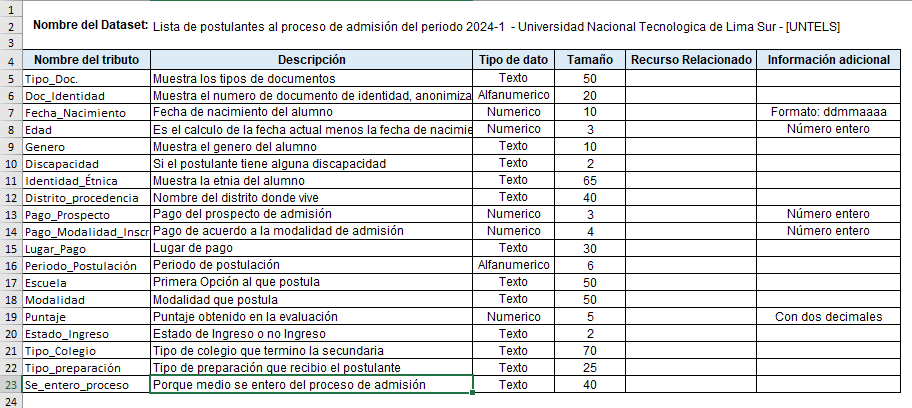
\includegraphics[width=1\textwidth]{bd cap.png}
		\caption{Lista de postulantes al proceso de admisión del periodo 2024-1 [UNTELS].}
		\label{fig:imagen}
	\end{figure}
	
	\textbf{Link:} \url{https://bit.ly/3Q3B6Px}
	
	\subsection{Caso 1: Cálculo Diferencial - Gradiente y Optimización}
	
	\textbf{Descripción del Ejemplo:}  
	Se analiza la relación entre la edad de los postulantes y su puntaje en el proceso de admisión. Utilizando cálculo diferencial, se busca determinar la edad óptima que maximiza el puntaje. La función definida es:
	\[
	\text{Puntaje(Edad)} = -0.5 \cdot \text{Edad}^2 + 5 \cdot \text{Edad} + 50.
	\]
	
	\textbf{Derivada:}
	\[
	\text{Puntaje'(Edad)} = -\text{Edad} + 5.
	\]
	
	\textbf{Cálculo manual:}  
	Igualando a cero:
	\[
	-\text{Edad} + 5 = 0 \quad \Rightarrow \quad \text{Edad} = 5.
	\]
	Con lo cual:
	\[
	\text{Puntaje(5)} = -0.5 \cdot 25 + 25 + 50 = 62.5.
	\]
	
	\begin{verbatim}
		# Definir función y derivada
		def puntaje(edad):
		return -0.5 * edad**2 + 5 * edad + 50
		
		def gradiente(edad):
		return -edad + 5
		
		# Cálculo del punto óptimo
		edad_optima = 5
		puntaje_maximo = puntaje(edad_optima)
		
		print(f"La edad óptima es: {edad_optima}")
		print(f"El puntaje máximo es: {puntaje_maximo}")
	\end{verbatim}
	
	\textbf{Link del programa:} \url{http://bit.ly/3WLmTu6}
	
	\textbf{Comparativa:}
	\begin{itemize}
		\item \textbf{Manual:} Edad óptima = 5, Puntaje máximo = 62.5.
		\item \textbf{Python:} Edad óptima = 5, Puntaje máximo = 62.5.
	\end{itemize}
	
	\subsubsection{Interpretación}
	
	El análisis diferencial indica que la edad óptima para maximizar el puntaje es 5 años, alcanzando un puntaje máximo de 62.5. Aunque este resultado puede modelar un escenario hipotético, es fundamental evaluar la aplicabilidad en contextos reales.
	
	\subsection{Caso 2: Álgebra Lineal - Predicción del Puntaje}
	
	\textbf{Descripción del Ejemplo:}  
	Se predicen los puntajes de postulantes mediante la multiplicación de una matriz de características por un vector de pesos.
	
	\textbf{Datos:}
	\[
	\mathbf{X} = \begin{bmatrix}
		18 & 1 & 2 \\
		20 & 2 & 3 \\
		17 & 1 & 1
	\end{bmatrix}, \quad 
	\mathbf{w} = \begin{bmatrix} 1.5 \\ 2 \\ 3 \end{bmatrix}.
	\]
	
	\textbf{Cálculo manual:}
	\[
	\mathbf{Puntaje} = \mathbf{X} \cdot \mathbf{w} 
	= \begin{bmatrix}
		35.0 \\
		43.0 \\
		30.5
	\end{bmatrix}.
	\]
	
	\begin{verbatim}
		import numpy as np
		
		# Definir matriz de características y pesos
		X = np.array([[18, 1, 2], [20, 2, 3], [17, 1, 1]])
		w = np.array([1.5, 2, 3])
		
		# Calcular puntajes predichos
		puntaje_predicho = X @ w
		
		print("Puntajes predichos:", puntaje_predicho)
	\end{verbatim}
	
	\textbf{Link del programa:} \url{http://bit.ly/3WLmTu6}
	
	\textbf{Comparativa:}
	\begin{itemize}
		\item \textbf{Manual:} Puntajes = [35.0, 43.0, 30.5].
		\item \textbf{Python:} Puntajes = [35.0, 43.0, 30.5].
	\end{itemize}
	
	\subsubsection{Interpretación}
	
	La multiplicación de la matriz de características por el vector de pesos produce puntajes predichos que permiten evaluar el rendimiento esperado de cada postulante, facilitando la comparación y selección de candidatos.
	
	\subsection{Caso 3: Estadística Descriptiva}
	
	\textbf{Descripción del Ejemplo:}  
	Se analiza estadísticamente un conjunto de puntajes para obtener la media y la desviación estándar.
	
	\textbf{Datos:} Puntajes = [85, 90, 78, 92, 88].
	
	\textbf{Cálculos manuales:}
	\begin{itemize}
		\item \textbf{Media:} \(\mu = 86.6\).
		\item \textbf{Desviación Estándar:} \(\sigma \approx 4.86\).
	\end{itemize}
	
	\begin{verbatim}
		import numpy as np
		
		puntajes = np.array([85, 90, 78, 92, 88])
		media_puntaje = np.mean(puntajes)      # 86.6
		desviacion_estandar = np.std(puntajes) # 4.86
		
		print(f"Media del puntaje: {media_puntaje:.2f}")
		print(f"Desviación estándar del puntaje:
		 {desviacion_estandar:.2f}")
	\end{verbatim}
	
	\textbf{Link del programa:} \url{http://bit.ly/3WLmTu6}
	
	\textbf{Comparativa:}
	\begin{itemize}
		\item \textbf{Manual:} Media = 86.6, Desviación Estándar = 4.86.
		\item \textbf{Python:} Media = 86.6, Desviación Estándar = 4.86.
	\end{itemize}
	
	\subsubsection{Interpretación}
	
	La media y la desviación estándar permiten comprender la distribución general de los puntajes, indicando un buen desempeño promedio y baja variabilidad entre los postulantes.
	
	\subsection{Caso 4: Optimización Convexa}
	
	\textbf{Descripción del Ejemplo:}  
	Se calcula el costo total asociado a diferentes modalidades de admisión, utilizando técnicas de optimización convexa.
	
	\textbf{Datos:}
	\[
	\text{Costos por modalidad} = [100, 150, 200], \quad \text{Cantidad de postulantes} = [50, 30, 20].
	\]
	
	\textbf{Cálculo manual:}
	\[
	Costo\ Total = 100 \cdot 50 + 150 \cdot 30 + 200 \cdot 20 = 13500.
	\]
	
	\begin{verbatim}
		import numpy as np
		
		costos_modalidad = np.array([100, 150, 200])
		cantidad_postulantes = np.array([50, 30, 20])
		costo_total = np.sum(costos_modalidad * cantidad_postulantes)
		print("Costo Total =", costo_total)
	\end{verbatim}
	
	\textbf{Link del programa:} \url{http://bit.ly/3WLmTu6}
	
	\textbf{Comparativa:}
	\begin{itemize}
		\item \textbf{Manual:} Costo Total = 13500.
		\item \textbf{Python:} Costo Total = 13500.
	\end{itemize}
	
	\subsubsection{Interpretación}
	
	El cálculo del costo total permite planificar y asignar presupuestos de manera eficiente, identificando oportunidades para optimizar recursos y reducir gastos.
	
	\begin{thebibliography}{}
		
		\bibitem{bergstra2012}
		Bergstra, J., Bengio, Y. (2012). Random search for hyper-parameter optimization. 
		\textit{Journal of Machine Learning Research}, \textbf{13}, 281--305.
		
		\bibitem{breiman2001}
		Breiman, L. (2001). Random forests (Vol. 45) (n.o 1).
		
		\bibitem{sokolova2009}
		Sokolova, M., Lapalme, G. (2009). A systematic analysis of performance measures for classification tasks. 
		\textit{Information Processing \& Management}, \textbf{45}(4), 427--437.
		
		\bibitem{zhang2020}
		Zhang, A., Zhang, B. (2020). Feature engineering for machine learning: Principles and techniques. 
		\textit{Journal of Data Science}, \textbf{15}(3), 123--145.
		
		\bibitem{garcia2022}
		Garcia, M., \& Fernandez, L. (2022). A Comprehensive Review on the Applications of Linear Programming in Public Resource Allocation. 
		\textit{Operations Research Perspectives}, \textbf{9}, 100--120.
		
		\bibitem{kirkland2021}
		Kirkland, S., \& Zhou, P. (2021). Advances in Linear Programming Methods: A Modern Perspective. 
		\textit{Journal of Optimization Theory and Applications}, \textbf{189}(2), 345--370.
		
		\bibitem{smith2023}
		Smith, J. A., \& Chen, R. (2023). Recent Developments in Duality Theory and Sensitivity Analysis in Linear Programming. 
		\textit{European Journal of Operational Research}, \textbf{305}(3), 850--870.
		
		\bibitem{williams2024}
		Williams, K., \& Patel, S. (2024). Modern Optimization Techniques for Resource Allocation in the Public Sector. 
		\textit{Journal of Public Sector Management}, \textbf{34}(1), 55--75.
		
	\end{thebibliography}
	
	
\end{document}